%% bare_jrnl.tex
%% V1.4b
%% 2019/08/26
%% by Vasileios Koulis
%% see http://www.michaelshell.org/
%% for current contact information.
%%



\documentclass[journal]{IEEEtran}
\usepackage[pdftex]{graphicx}
\usepackage{url}

\begin{document}

\title{ROS Robot - Weed Spray}
\author{Vasileios Koulis\\~\IEEEmembership{University of Lincoln}\\18710208@students.lincoln.ac.uk}

\markboth{Robot Programming Assessment Item 2 - REPORT, December~2019}{}

\maketitle


\begin{abstract}
Using ROS for controlling a Thorvald robot to spray the weeds in row structured crops using a downward looking camera to identify them.
\end{abstract}


% ----------------
\section{Introduction}
All farmers have to deal with weeds for their crops because they are bad for the growth of plant, so they need to be removed by various methods. Normally farmers have to go all around the field with vehicles and spray all the areas that have no crops. With robots this procedure can be automated by targeting specific locations with computer vision. 

There are numerous benefits for looking into agricultural robots like the one we are using (Thorvald):

\begin{itemize}
  \item Increased productivity
  \item decreased production costs with the best use of resources and minimal environmental damage
  \item Reduce the chemicals used
  \item Early detection and elimination of weeds 
  \item Identify complex shapes of weeds
  \item Easier to use through automated procedures
\end{itemize}

In this paper I am focusing on the weed identification using a camera on board of a Thorvald robot in a virtual environment using ROS. All information is stored in a pointCloud so that it can be used to spray the weeds as it passes through each row of crop. Each row has a different crop which include \textbf{onions}, \textbf{cabbages} and \textbf{basils} Fig. \ref{orig_plants}.

Some characteristics of the robot are really important to have. One of them is to be omnidirectional so that it will be able to move each tire individually because inside the field it must make manoeuvres to get the desired position. It must also have a camera so that the recognition program can use it to identify the desired object. One more important is the GPS so that it can understand where exactly it is.

\begin{figure}[ht]
\centering
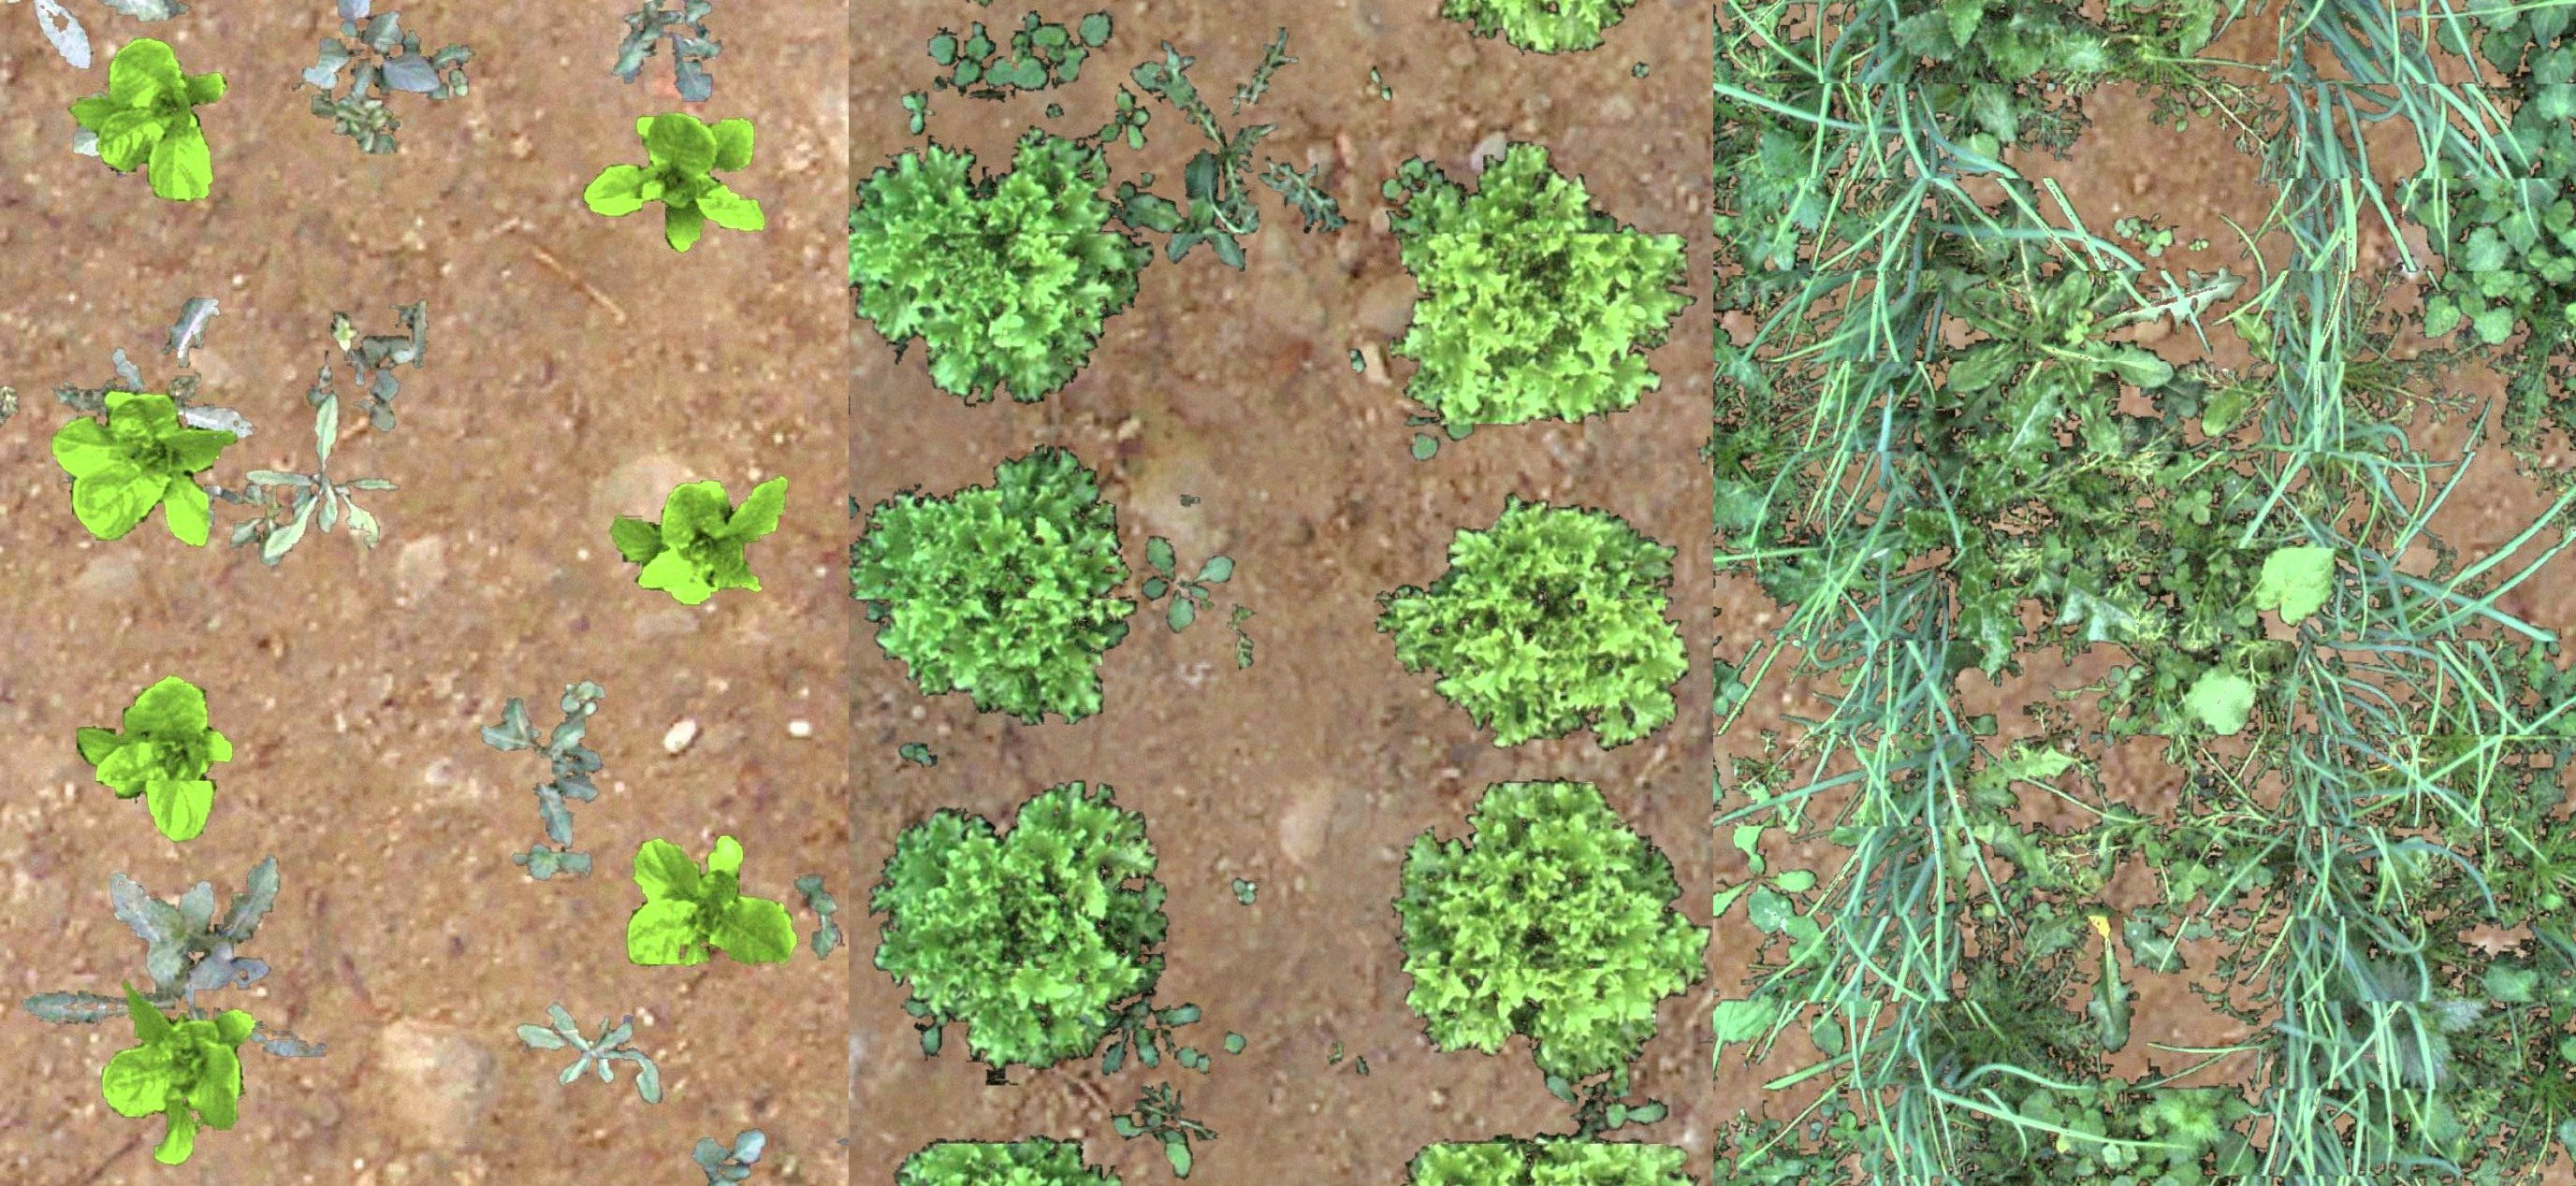
\includegraphics[width=3.2in]{originalplants}
\caption{Rows of crops provided.}
\label{orig_plants}
\end{figure}

\begin{figure}[ht]
\centering
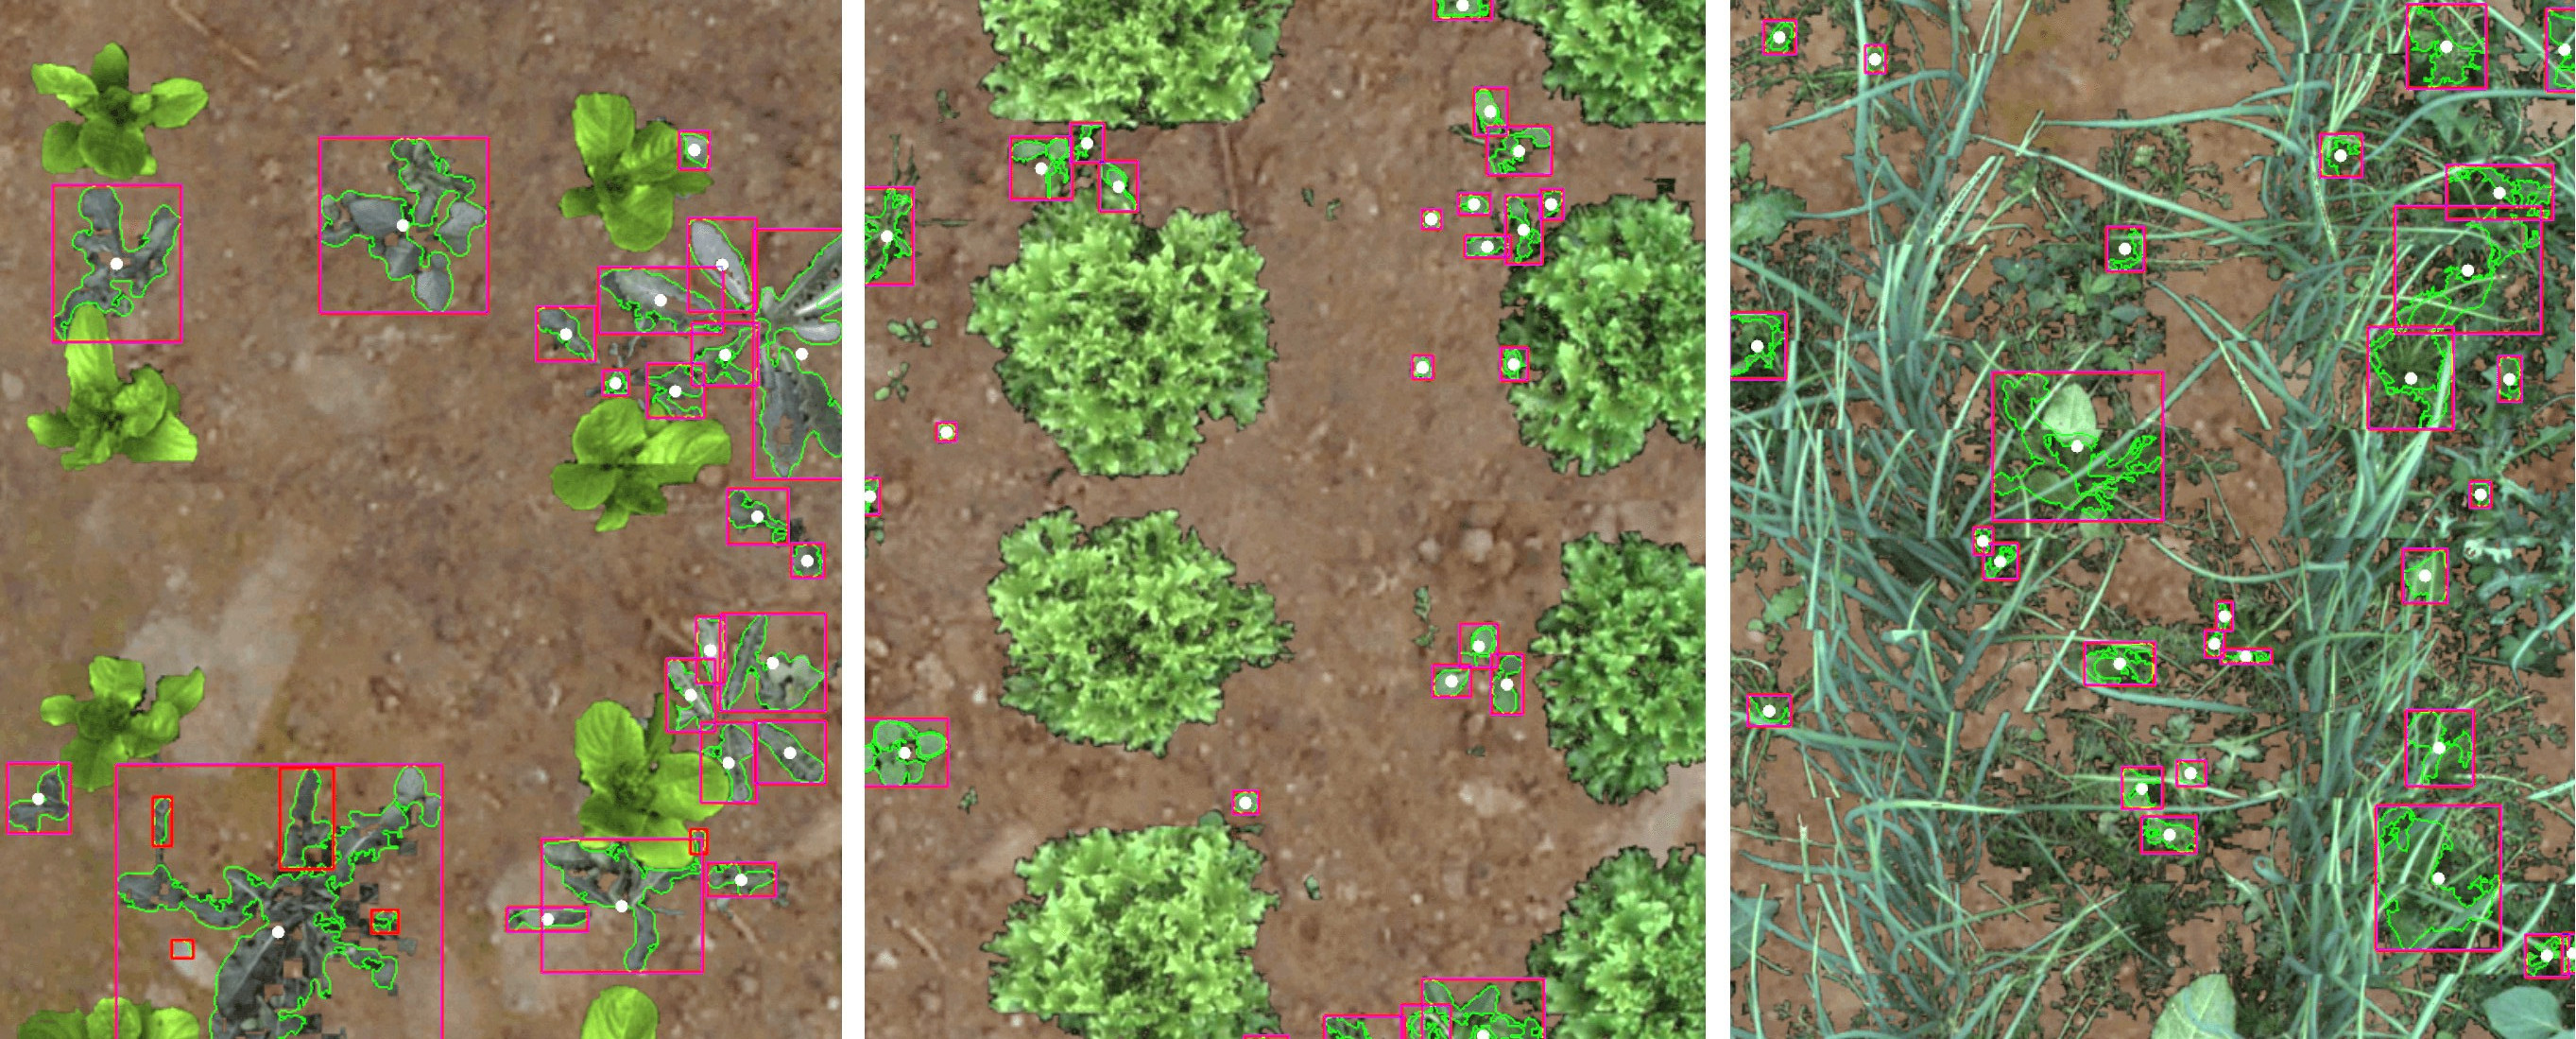
\includegraphics[width=3.5in]{processedplants}
\caption{Rows of crops with their canopy and points.}
\label{proc_plants}
\end{figure}


% \newpage

% ----------------
\section{Related Work}
A lot of research has been done for dealing with weed control. All of them are relying on a camera and image recognition with different approaches each.

On this paper \cite{weed_control2} it focuses on the weeds for tomatoes using alternative methods. It uses mechanical ways to deal with them and for the weed recognition it uses a camera by training a model for the specific weeds. The amount of weeds it could find was around 70\% in a real-time system.

On this paper \cite{weed_control3} is using support vector machines for automatically spraying. It compares different image processing techniques and they used images that were 60x60 with a total of 1200 images. They also did a classification and found out that using the SWLDA (step-wise  linear  discriminant  analysis) technique the accuracy was 98.1\% which was much better than other studies.

On this paper \cite{weed_control4} it is identifying the type of weeds which helps determine the type of chemical product to use. Also finds the growth stage and the location in the field. It uses a colour matching method on the leafs to determine what the weed and after that they segmentate them. 

On this paper \cite{weed_control5} it is using colour matching in different light conditions. This is done by identifying the rows of crop and based on the colours of this, it can identify the weed. it concludes that this technique is more accurate than BP and SVM algorithms.

On this paper \cite{weed_control5} it focuses on multi-spectal reflectance gathering. This is done by sending a light ray into an area and then get the reflection into a monochrome camera. The problem with this technique is that it is very slow because of the camera frame rate.


% ----------------
\section{Implementation}
Obtaining all the weeds is really difficult because there are many types of weeds and the weather conditions might change from area to area. The colour matching approach is working fine on the provided dataset with predefined colours, but in the real world the result will not be as we want it. 

There are other approaches that provide results that are working on a more broad data, though they are more difficult to implement. The one I used is the Mask-RCNN which uses Neural Network but it requires to annotate the weeds manually which is a very difficult job to do so this is why I used it only for the weeds on the cabbages.

After the annotation was done, I had to train the dataset which took more than 35 hours to finish and after it was done the evaluation process for each image took more than 3 seconds to be completed.

\begin{figure}[ht]
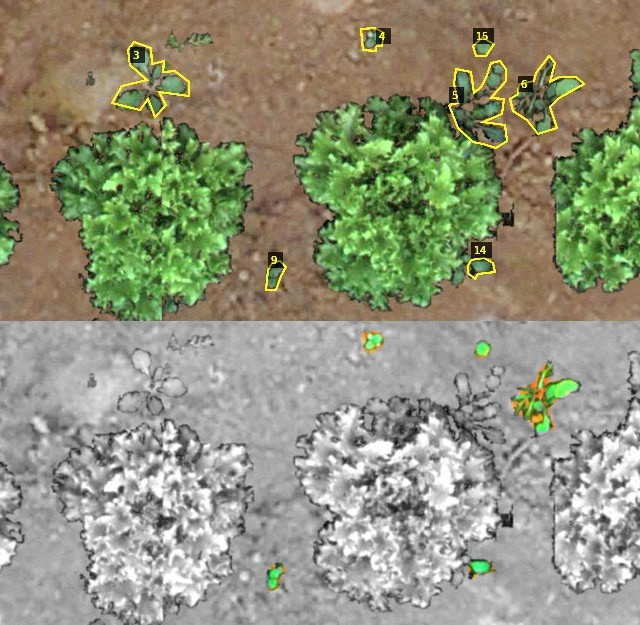
\includegraphics[width=3in]{cnn}
\caption{Annotation of images (top), result of the RCNN evaluation (bottom).}
\label{annotation_cnn}
\end{figure}

After checking the result of the RCNN method, I decided to go with the colour matching because it was much faster for a real time application. To make it more modular, the application is divided into the following nodes:

\subsection{Image Recognition}
For the weed extraction I am using OpenCV which finds all the necessary objects through HSV image matching. These are the steps it takes:
\begin{itemize}
  \item Removes the Background.
  \item Extracts the canopy of the weed.
  \item Removes the smallest canopies that are bellow a threshold.
  \item Finds the middle point.
  \item Rectify each point with the camera lens.
  \item Converts all points into real map coordinates.
  \item Publish as a pointCloud to a specific topic.
\end{itemize}
The final result from the weed extraction is published as an image and you can see on Fig. \ref{proc_plants}.

\subsection{GetPoints}
At this step a new node is responsible for deciding what to do all the points:
\begin{itemize}
  \item Gets each published pointCloud and filters the duplicates.
  \item Checks if the sprayer is on top of one of these points and activates the spraying.
  \item Publishes the points so that it will be visualised on Rviz.
\end{itemize}

\subsection{Moving}
For moving the robot way-points had to be defined at the start and at the end of each line of crops. These were defined manually using world coordinates. The node waits for the robot to move into the next way-point using move base and then continues to the next one. When it is on top of a specific line of crops, it publishes the type of plant so that it can be used by the image recognition node.

\begin{figure}[ht]
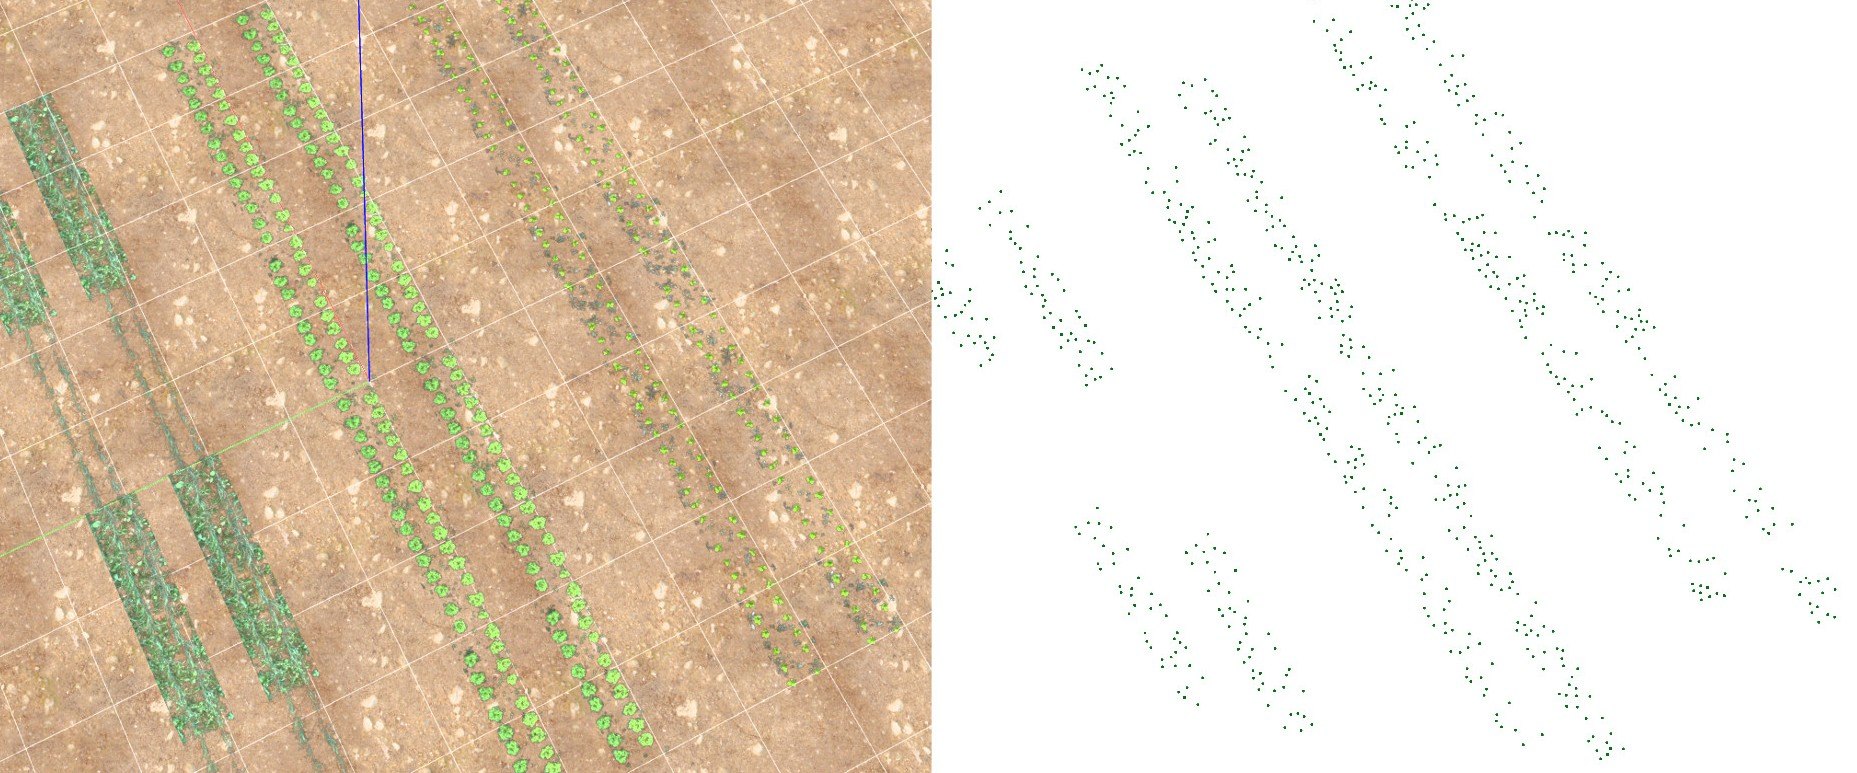
\includegraphics[width=3.5in]{allweeds}
\caption{Original crops (left) and the recognised weeds (right).}
\label{all_weeds}
\end{figure}



% ----------------
\section{Conclusion}
By providing specific images it is very easy and fast to make colour matching to get the result it is needed, although by training a model with some datasets of weeds it becomes more dynamic and can be used on more environments.

The RCNN model I created didn't have the expected result, as it didn't find all the plants and it was really slow to get the results. On the other hand the colour matching was so fast that it can in real time get all the weeds and do all the transformations so that they could be sprayed.

One problem emerged which had to do with the transformation of points to real world coordinates. All the points are shifted because the robot is constantly moving and the transformation is done at the future position of the robot and not at the moment that the weeds were detected.




\begin{thebibliography}{}
% BPG 11: Weed control\\ \url{https://www.forestresearch.gov.uk/research/best-practice-guidance-for-land-regeneration/}
\bibitem{maskcnn}
Mask RCNN \url{https://github.com/matterport/MaskRCNN}

\bibitem{weed_control1}
Forest Research, “Weed Control,” The Land Regeneration and Urban Greenspace Research Group., 2014.
\bibitem{weed_control2}
W. S. Lee, D. C. Slaughter, and D. K. Giles, “Robotic Weed Control System for Tomatoes,” Precis. Agric., 1999.
\bibitem{weed_control3}
M. H. Siddiqi, S. W. Lee, and A. M. Khan, “Weed image classification using wavelet transform, stepwise linear discriminant analysis, and support vector machines for an automatic spray control system,” J. Inf. Sci. Eng., 2014.
\bibitem{weed_control4}
A. G. Manh, G. Rabatel, L. Assemat, and M. J. Aldon, “Weed leaf image segmentation by deformable templates,” J. Agric. Eng. Res., 2001.
\bibitem{weed_control5}
J. L. Tang, X. Q. Chen, R. H. Miao, and D. Wang, “Weed detection using image processing under different illumination for site-specific areas spraying,” Comput. Electron. Agric., 2016.
\bibitem{weed_control6}
F. Feyaerts and L. Van Gool, “Multi-spectral vision system for weed detection,” Pattern Recognit. Lett., 2001.
\end{thebibliography}
% ----------------

% \section {TO DELETE}
% \begin{itemize}
%   \item \textbf{\textit{The aim and specific objectives of your developed artefact, including some motivation as to why this artefact has some significance;}}
%   \item \textbf{\textit{Related work, referring to other researchers’ works on a similar task, and discussing these in the direct context to your work;}}
%   \item \textbf{\textit{The concept of your system architecture and the choice of algorithms or components you made to develop your artefact. You should back your justification with academic references to make a clear argument for your design choices;}}
%   \item \textbf{\textit{The evaluation of the artefact using appropriate quantitative methodology. Your evaluation must be focused on your chosen focus area, i.e. either perception, navigation or coordination. You must adopt suitable evaluation metrics and methodologies established in the field, reflecting the chosen focus area.}}
% \end{itemize}


% that's all folks
\end{document}



